%!TEX root = ..\main.tex
\subsection{Simulation details and equilibrium results}
\label{subsec:simulation_details}

Defining $\rho = \frac{N D}{L}$ where $N$ --- number of particles and $D = \Delta z_{min}$ --- particle diameter calculated numerically, we immediately obtain the simulation system size $L = N D/ \rho$. In our simulations we considered cases of different densities $\rho = (0.25,\ 0.5,\ 0.75)$.

To check for existence of finite-size effects, we performed simulations with different system sizes $N = (1600,\ 3200,\ 6400)$, keeping the same density.

The Monte Carlo simulations were allowed to equilibrate for $\Delta = 3 \cdot 10^5$ Monte Carlo sweeps, and different quantities were measured after every $\Delta$ sweeps, obtaining $10$ uncorrelated samples. To generate the initial configuration, dipolar particles were regularly distributed along $z$ axis, with an interparticle distance $d = \frac{D}{\rho}$, and then displaced by a certain value, following a uniform distribution in the range $[-d/4, d/4]$. The orientation of the dipoles was generated uniformly at random.

\subsection{Equilibrium results}
\label{subsec:monte_carlo_results}
First, we study how the nematic order parameter $S$ depends $k_BT$ at equilibrium for different system densities. The $S$ is defined as
\begin{equation}
\label{eq:nematic_order_parameter}
	S = \frac{3 \langle\cos^2 \theta\rangle - 1}{2}
	,
\end{equation}
where $\theta$ it the angle between particle dipole moment and $z$ axis, while angle brackets denote ensemble averages over all particles.

As we can see on the Figure~\ref{fig:op_kbt}, the nematic order increases with decrease of $k_BT$. The results presented are averaged over $400$ samples. 

For high density we observe exponential decrease in ordering with increase in $k_BT$, however, for lower densities, the relation is more complex. For the low $k_BT$ the decrease in ordering is faster then in case of high density, however, for higher $k_BT$ the decrease in order parameter slows down.  

Additionally, there is no systematic scaling with system size, which indicates the absence of finite size effects. The results presented here are consistent with reported in literature (see~\cite{Marshall2015}). We must also note that statistical errors observed are of order $10^{-3}$. In the section~\ref{sec:langevin_dynamics} we will discuss LD~system relaxation towards the equilibrium results.

\begin{figure}[h]
\centering
	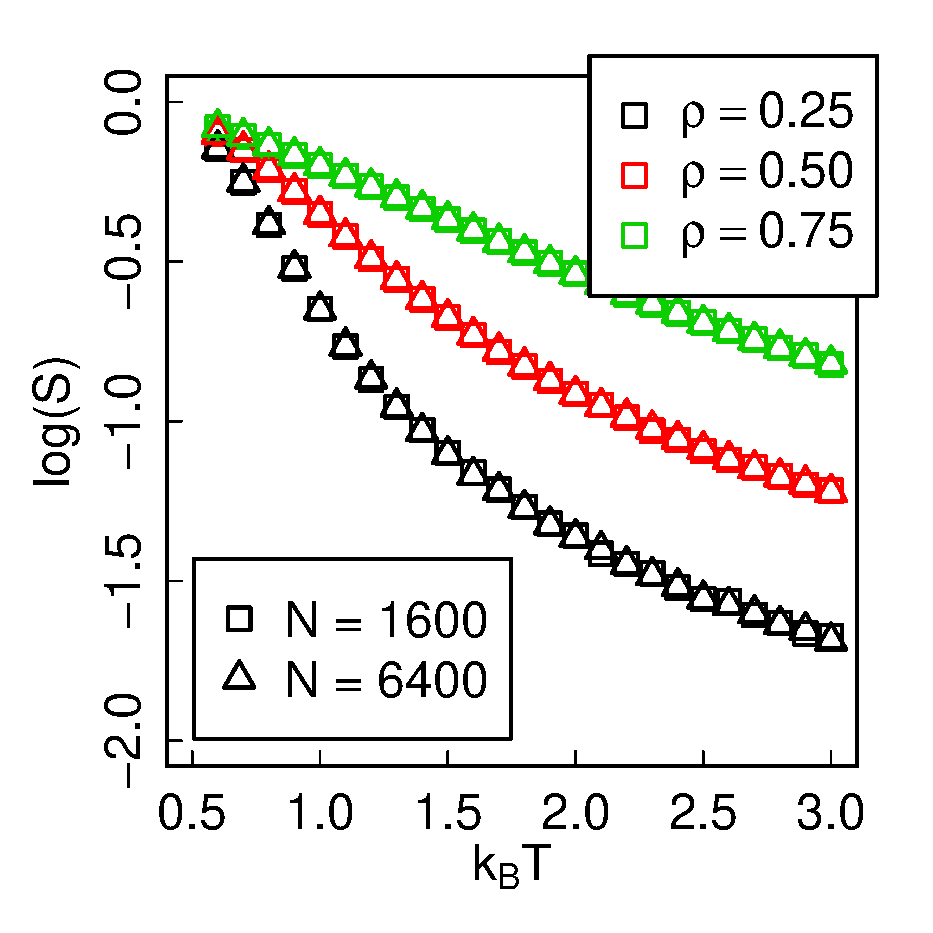
\includegraphics[width=0.5\textwidth]{Images/op_eq_log}
	\captionsetup{justification=centering, width=0.9\columnwidth}
	\caption{Order parameter defined by Eq.~\eqref{eq:nematic_order_parameter} versus $k_BT$ for Monte-Carlo simulations. Triangles shows results for $N = 6400$ and squares for $N = 1600$ particles. As we can see there is no systematic scaling with system size. The results are obtained by means of MC simulations, and are average over $200$ samples as described in sec.~\ref{subsec:simulation_details}}
	\label{fig:op_kbt}
\end{figure}

To characterize the dependence of the structure on $k_BT$, we analyze the orientation correlation of particles as function of distance between them:
\begin{equation}
\label{eq:distance_correlation}
	C(\Delta z) = \langle\cos \theta_i \cos \theta_j\rangle
	,
\end{equation}
where $\theta_i$ and $\theta_j$ are angles between spatial axis and dipole moments of particles for which $\Delta z - \delta < |z_j - z_i| \leq \Delta z + \delta$, where $2\delta$ is a predefined space sampling. Angle brackets denotes ensemble-averaging over all particles in all samples which satisfy distance criteria.

For all observed range of simulation parameters the correlation decays exponentially with distance. For selected number of simulation parameters the results are presented at the Figure~\ref{fig:dist_corr_eq}, done in log-linear scale. The dots are obtained with space sampling $\delta = 0.25D$, and are averaged over $400$ samples with $N = 6400$ particles. Lines are obtained by doing best linear fit to the results in range $0.01 < C(\Delta z) < 0.45$.
\begin{figure}[t]
\centering
\begin{subfigure}[t]{0.32\textwidth}
	\centering
	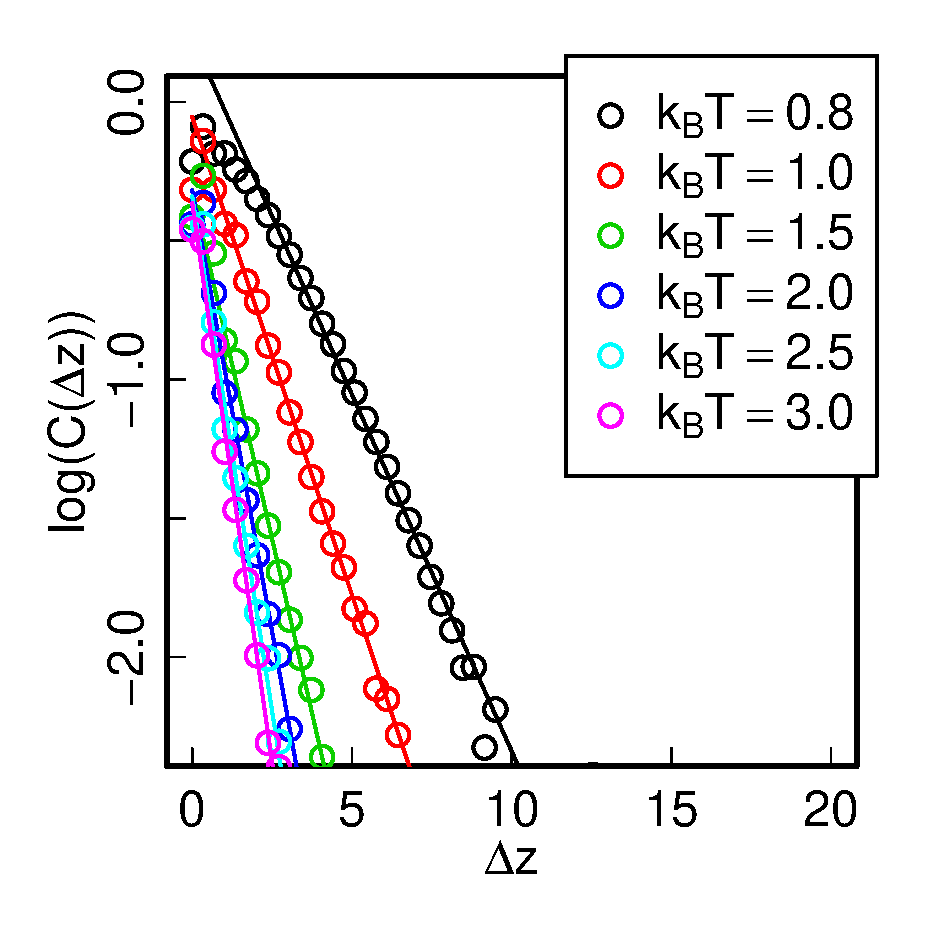
\includegraphics[width=\textwidth]{Images/distCor_25}
\end{subfigure}
\begin{subfigure}[t]{0.32\textwidth}
	\centering
	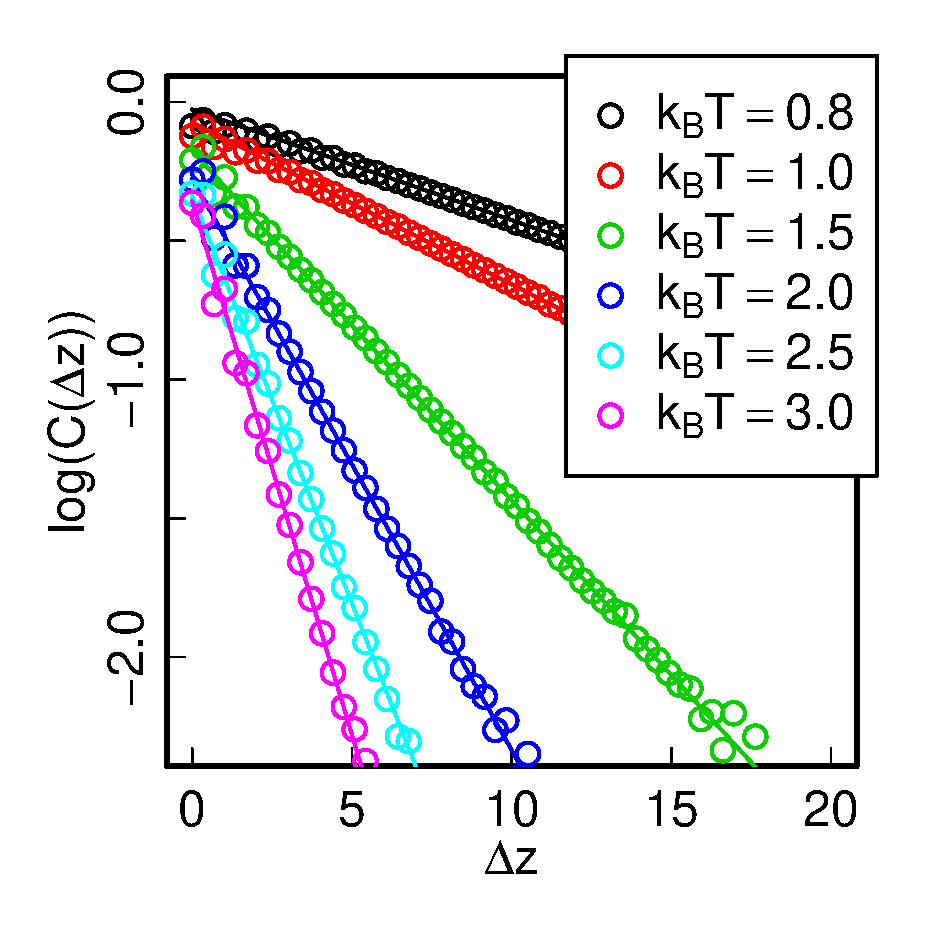
\includegraphics[width=\textwidth]{Images/distCor_75}
\end{subfigure}
\begin{subfigure}[t]{0.32\textwidth}
	\centering
	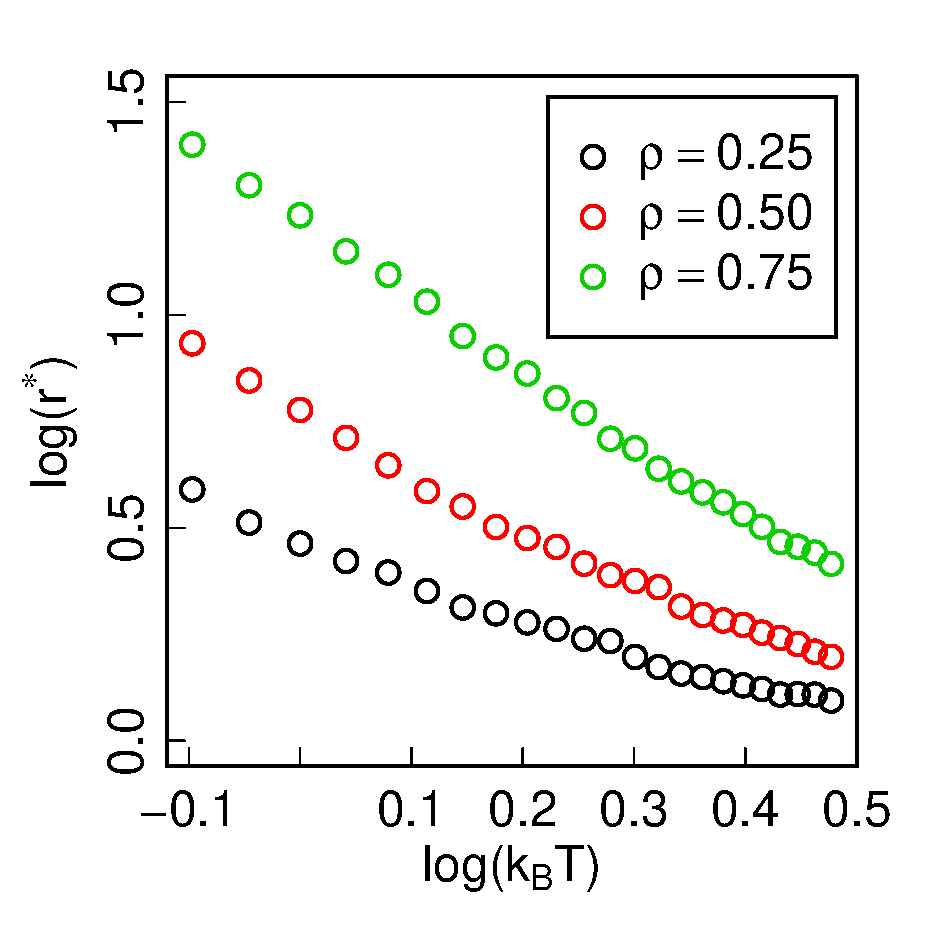
\includegraphics[width=\textwidth]{Images/correlation_length_eq}
\end{subfigure}
	\captionsetup{justification=centering, width=0.9\columnwidth}
	\caption{Orientation correlation as function of distance defined by Eq.~\eqref{eq:distance_correlation} at equilibrium for $\rho = 0.25$ (left) and $\rho = 0.75$ (center). The points are calculated for simulations with $N = 6400$ particles and the results are averaged over $400$ samples as described in sec.~\ref{subsec:simulation_details}. Lines are the best linear fit to the results in range $0.01 < C(\Delta z) < 0.45$. (Right) shows $r^*$ as defined in \eqref{eq:slopes_def}.}
	\label{fig:dist_corr_eq}
\end{figure}

The exponential decay of correlation with length for every combination of simulation parameters shows that we do not have any critical transition occurring in the system under study, despite non-zero order parameter observed above.

We could now write $C(\Delta z)$ as
\begin{equation}
	\label{eq:slopes_def}
	C(\Delta z) \propto \exp\left[-\frac{\Delta z}{r^*(k_BT, \rho)} \right]
\end{equation}
where $r^*$ is the correlation length and depends on the system density and $k_BT$. The dependence of $r^*$ on the $k_BT$ for different system densities is shown at the Figure \ref{fig:dist_corr_eq_slopes}. We must note the similarity in behavior of order parameter and the correlation distance, however, the obtained results suggest slow (power-law) increase in correlation distance with decrease in $k_BT$.

%\begin{figure}[h]
%\centering
%\begin{subfigure}[t]{0.5\textwidth}
%	\centering
%	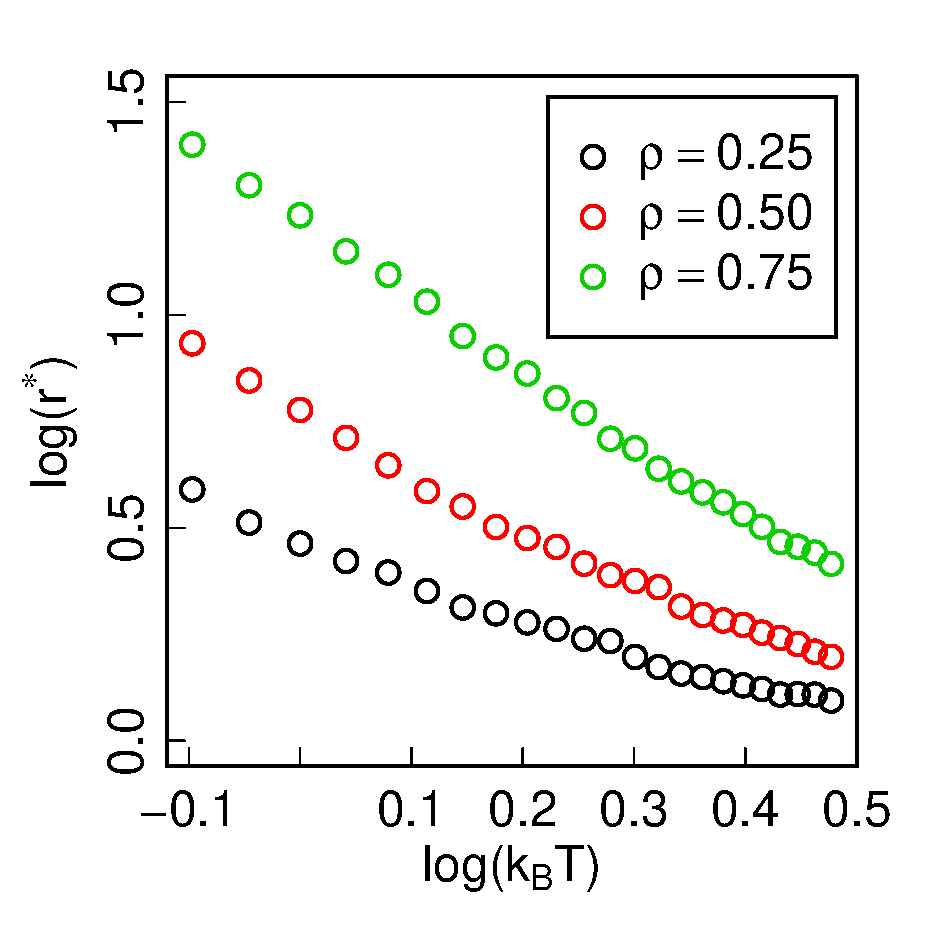
\includegraphics[width=\textwidth]{Images/correlation_length_eq}
%\end{subfigure}
%	\captionsetup{justification=centering, width=0.9\columnwidth}
%	\caption{$r^*$ as defined in \eqref{eq:slopes_def}, obtained as inverse slope of orientation correlation shown at Figure~\ref{fig:dist_corr_eq}.}
%	\label{fig:dist_corr_eq_slopes}
%\end{figure}
